\documentclass[letterpaper, 10 pt, conference]{sty/ieeeconf}

\IEEEoverridecommandlockouts

\overrideIEEEmargins

\usepackage{graphics}
\usepackage{epsfig}
\usepackage{amsmath}
\usepackage{amssymb}
\usepackage{txfonts}
\usepackage{tikz}
\usepackage[T1]{fontenc}

\DeclareMathOperator*{\argmax}{arg\,max}
\DeclareMathOperator*{\argmin}{arg\,min}

\begin{document}

\title{\LARGE \bf
Bayesian On-line Learning of Driving Behaviors
}

\author{
\authorblockN{
J\'{e}r\^{o}me Maye\authorrefmark{1},
Rudolph Triebel\authorrefmark{1},
Luciano Spinello\authorrefmark{2},
and Roland Siegwart\authorrefmark{1}
}
\authorblockA{
\authorrefmark{1}
Autonomous Systems Lab, ETH Zurich, Switzerland\\
email: \{jerome.maye, rudolph.triebel, roland.siegwart\}@mavt.ethz.ch}
\authorblockA{
\authorrefmark{2}
Social Robotics Lab, University of Freiburg, Germany\\
email: spinello@informatik.uni-freiburg.de}
}

\maketitle

\begin{abstract}
This paper presents a novel self-supervised online learning method to
discover driving behaviors from data acquired with an inertial
measurement unit (IMU) and a camera. Both sensors where mounted in a
car that was driven by a human through a typical city environment with
intersections, pedestrian crossings and traffic lights. The presented
system extracts motion segments from the IMU data and relates them to
the visual cues obtained from the camera data. It employs a Bayesian
on-line estimation method to discover the motion segments based on
change-point detection and uses a Dirichlet Compound Multinomial (DCM)
model to represent the visual features extracted from the camera
images. By incorporating these visual cues into the on-line estimation
process, labels are computed that are equal for similar motion
segments. As a result, typical traffic situations such as braking
maneuvres in front of a red light can be identified
automatically. Furthermore, appropriate actions in form of observed
motion changes are associated to the discovered traffic
situations. The approach is evaluated on a real data set acquired in
the center of Zurich.

%One research area that has turned more and more into the focus of
%interest during the last years is the development of driver
%intelligent assistant systems. In particular, a very active topic is
%the design of human-friendly vehicle control systems, able to meet the
%driver specific behaviors. In this paper we address the problem of
%learning driver behaviors based on on camera images and inertial
%information (IMU). Our approach proposes a novel on-line and
%unsupervised way of learning driver's behavior in different traffic
%conditions.  Specifically we learn the relationship between vehicle
%motion and image streams.  In this paper we introduce a novel
%technique that uses a \textit{change-point} detection model to segment
%IMU and image streams into portions corresponding to
%behaviors. Change-point detection is the problem of detecting abrupt
%changes to the parameters of a statistical model. This is computed
%on-line and in an unsupervised manner. The results from experiments in
%populated urban environments demonstrate the robustness of the
%algorithm to correctly identify several driving behaviors.

\end{abstract}

\section{Introduction}
One research area that has turned more and more into the focus of interest
during the last years is the development of driver intelligent assistant
systems. In particular, a very active topic is the design of human-friendly
vehicle control systems, able to meet the driver specific behaviors. In this
paper we address the problem of learning driver behaviors by using multiple
sensing modalities, namely camera images and inertial information (IMU). Most
existing techniques build a behavior model from heuristic rules or from
supervised training data. Our approach proposes a novel Bayesian on-line and
unsupervised way of learning driver's behavior in different traffic conditions.
Specifically we learn the relationship between vehicle motion and image streams.

Motion data is segmented by using a \textit{change-point} detection method, a
technique that solves the problem of detecting abrupt changes to the parameters
of a statistical model. We use a Bayesian approach to compute the probability of
a change-point occurring at each time step. We have formulated a fast
approximation of this method by using a Rao-Blackwellized particle filter.
The motion segments are grouped together to represent traffic situations by
exploiting similarity in the associated image streams. This is computed on-line
and in an unsupervised manner. The streams are represented as collection of
bag-of-words modeled after a Dirichlet Compound Multinomial model. This process
provides tools to predict the driving actions conditioned on the current traffic
situation.

The the paper is structured as follows. Section~\ref{sec:related}
summarizes the previous work related to ours. Section~\ref{sec:motion}
describes our motion segmentation method. Section~\ref{sec:labeling}
shows how we model a traffic situation. Section~\ref{sec:action} demonstrates
our action model. Section~\ref{sec:exp} presents experimental results.
Section~\ref{sec:conc} outlines our conclusions and provides some insights for
future work.


\section{Related Work\label{sec:related}}
Existing driving behavior models in psychology are largely subjective and based
on self-report scales~\cite{ranney94models}. They are difficult to quantify
because they include many psychological aspects like motivation, or risk
assessment.

Many works in the intelligent vehicle
literature~\cite{donges78two,mcruer80human,hess90control,macadam81application}
focus on modeling the driver behavior via their steering behavior or road
tracking information or desired driver's path as source of behavior's
information. Other works recognize driver's intentions via Bayesian reasoning on
a complex input including the driver's current control actions and the traffic
environment surrounding them~\cite{oliver00graphical,liu01modeling}. To our
knowledge, there has been few research works that combine traffic scenario
recognition and action prediction in an on-line and unsupervised fashion.

Maye \emph{et al.}~\cite{maye10inferring} were able to infer an action from a
direction sign in an indoor environment with a semi-supervised approach
using vision and prerecorded robot actions. We extend this idea to outdoor,
remove any supervision, and predict vehicle actions in an on-line fashion.
Meyer \emph{et al.}~\cite{meyer09probabilistic} predicted traffic situations
using Hidden Markov Models (HMM). They however restricted their situations space
by modeling states with respect to surrounding vehicles (distance, speed,
bearing) and manually segment image sequences for initial estimates. In this
paper, we exclude any manual intervention in the process and use a more complete
set of variables for predicting states.
Other works  \cite{heracles10vision,pugeault10learning} make use of supervised 
offline classification methods for learning the relation between driving actions and 
visual features. The actions are manually annotated and discretized in the training phase.

Change-point detection is a well-known problem in statistics. The CUSUM detector
\cite{page54continuous} uses piece-wise segments of Gaussian mean with noise.
Our implementation is largely inspired on the statistical models presented
in~\cite{adams07bayesian,fearnhead07online} that are easily applicable to
conjugate-exponential models. Several other applications, specially in the field
of computer vision, have used change-point detection
\cite{zhai05general,cemgil05hybrid}. To the author best knowledge this paper
represents the first application in the field of learning driving behaviors 
with multimodal sensory data.


\section{Problem Formulation\label{sec:formulation}}
Given a vehicle equipped with an Inertial Measurement Unit (IMU) and a monocular
camera, we seek to learn the relation between motion and visual data in an
on-line and unsupervised manner. We shall follow an entirely probabilistic
approach and formulate the problem as the estimation of the joint filtering
distribution

\begin{equation}
\label{eqn:jointfiletering}
p(r_t,l_t,\mathbf{a}_t\mid\mathbf{z}_{1:t},\mathbf{c}_{1:t}),
\end{equation}

where $r_t$ represents the motion segment length at time $t$, $l_t$ the image
label at time $t$, $\mathbf{a}_t$ the predicted action at time $t$,
$\mathbf{z}_{1:t}$ the IMU measurements up to time $t$, and $\mathbf{c}_{1:t}$
the camera measurements up to time $t$.

Exploiting conditional independences in \eqref{eqn:jointfiletering} provides the
decomposition

\begin{equation}
\label{eqn:jointdecomposition}
p(r_t,l_t,\mathbf{a}_t\mid\mathbf{z}_{1:t},\mathbf{c}_{1:t})=
p(r_t\mid\mathbf{z}_{1:t})p(l_t\mid r_t,\mathbf{c}_{1:t})
p(\mathbf{a}_t\mid r_t,l_t).
\end{equation}

$p(r_t\mid\mathbf{z}_{1:t})$ corresponds to the motion segmentation of
Section~\ref{sec:motion}, $p(l_t\mid r_t,\mathbf{c}_{1:t})$ to the traffic situation
modeling of Section~\ref{sec:labeling}, and $p(\mathbf{a}_t\mid r_t,l_t)$ to the action
prediction model of Section~\ref{sec:action}.


\section{Bayesian On-line Segmentation of Motion Data\label{sec:motion}}
Our motion segmentation algorithm is based on \emph{change-point detection}. A
change-point is an abrupt variation in the generative parameters of sequential
data. An efficient Bayesian on-line method for detecting change-points has been
independently proposed by Adams and MacKay~\cite{adams07bayesian} and by
Fearnhead and Liu~\cite{fearnhead07online}. In the following, we first present
this method in general and then show how we apply it to the problem of
segmenting motion data.

\subsection{Change-Point Detection}
Suppose we are given a time-dependent sequence of observations $\mathbf{z}_1,
\mathbf{z}_2, \dots,\mathbf{z}_T$, where the $\mathbf{z}_t$ can be scalars or
vectors. Our goal is to find segments $s_1,s_2,\dots,s_N$ with
$s_n=[\mathbf{z}_{b_n},\dots,\mathbf{z}_{e_n}]$, where $e_n > b_n$ and
$b_n = e_{n-1}+1$ for $n=1,\dots,N$. We assume that all data points
$\mathbf{z}_{b_n},\dots,\mathbf{z}_{e_n}$ of a segment $s_n$ are independently
and identically distributed (i.i.d.) according to a parameterized statistical
model \mbox{$p(\mathbf{z}\mid \boldsymbol{\eta}_n)$}. The parameter vectors
$\boldsymbol{\eta}_1,\dots \boldsymbol{\eta}_N$ are also assumed to be i.i.d.
The computation of the segments is done on-line, i.e., at each time step $t$ a
decision is made whether $\mathbf{z}_t$ is added to the current segment
$s_n=[\mathbf{z}_{b_n},\dots,\mathbf{z}_{t-1}]$ or a new segment is started. As
shown above, we denote the length of the current segment as $r_t$. Thus, after
deciding on $\mathbf{z}_t$, we have either $r_t=r_{t-1}+1$ or $r_t=0$ in case we
start a new segment.

To determine whether time step $t$ is a change-point, we analyze the posterior
distribution of the segment length conditioned on the data observed so far,
i.e. $p(r_t\mid \mathbf{z}_{1:t})$. Using the product rule, this filtering
distribution can be written as

\begin{equation}
\label{eqn:posterior}
p(r_t\mid \mathbf{z}_{1:t})\propto p(r_t,\mathbf{z}_{1:t}).
\end{equation}

The joint distribution in \eqref{eqn:posterior} can be expressed as

\begin{eqnarray}
\label{eqn:joint}
p(r_t,\mathbf{z}_{1:t})\hspace{-0.2cm}&=& \hspace{-0.35cm}\sum_{r_{t-1}}p(r_t,
r_{t-1},\mathbf{z}_{1:t})\nonumber\\
&=&\hspace{-0.35cm}\sum_{r_{t-1}}p(r_t,\mathbf{z}_t\mid r_{t-1},
\mathbf{z}_{1:t-1})p(r_{t-1},\mathbf{z}_{1:t-1})\nonumber\\
&=&\hspace{-0.35cm}\sum_{r_{t-1}}p(r_t\mid r_{t-1})p(\mathbf{z}_t\mid r_{t-1},
\mathbf{z}_{1:t-1})p(r_{t-1},\mathbf{z}_{1:t-1}).
\end{eqnarray}

The right-hand side of \eqref{eqn:joint} consists of three terms: the
\emph{transition probability} $p(r_t\mid r_{t-1})$ of the Markov chain formed by
$r_1,r_2,\dots,r_t$, the \emph{predictive distribution}
$p(\mathbf{z}_t\mid r_{t-1},\mathbf{z}_{1:t-1})$, and the posterior
$p(r_{t-1},\mathbf{z}_{1:t-1})$ from the previous time step. We have exploited
the Markov assumption for the simplifications in \eqref{eqn:joint}.
%Fig.\ref{fig:model} illustrates \eqref{eqn:joint} with a graphical model.

%\begin{figure}[t]
%\centering
%\includegraphics[width=0.5\columnwidth]{fig/model.eps}
%\caption{Graphical model representation of the joint posterior
%  $p(r_t,\mathbf{z}_{1:t})$.}
%\label{fig:model}
%\end{figure}

As there are only two possible successor states for $r_t$, namely
\mbox{$r_{t-1}+1$} or $0$, we can model the transition probability using
statistical survival analysis, i.e., the segment length can
either ``survive'' or ``die''. To do this, we define a \emph{survival function}
$S(t)$ as the probability that the current segment is still alive after time
step $t$. The complement of $S$ is usually named the
\emph{lifetime distribution function} $F(t)= 1- S(t)$ and its temporal
derivative $f(t)$ is denoted the \emph{event rate}. Finally, the
\emph{hazard function} $h(t)$ is defined as the event rate conditioned on the
survival of the segment at time $t$, i.e.

\begin{equation}
\label{eqn:hazardfunc}
h(t) = \frac{f(t)}{S(t)} = \frac{f(t)}{1 - F(t)}.
\end{equation}

Intuitively, $h(t)$ represents the probability that the segment dies exactly at
the current time instant $t$. We can use $h(t)$ to model the transition
probability as

\begin{equation}
\label{eqn:transprob}
p(r_t\mid r_{t-1}) = \left\{
\begin{array}{l l}
h(r_{t-1}+1) & \quad \text{if $r_t=0$ }\\
1 - h(r_{t-1}+1) & \quad \text{if $r_t=r_{t-1}+1$}\\
0 & \quad \text{otherwise}.
\end{array} \right.
\end{equation}

A common approach is to model $S(t)$ as an exponential function
$S(t)=\exp(-\lambda t)$ with some given rate parameter $\lambda$. Then, the
hazard function turns into

\begin{equation}
\label{eqn:hazardexp}
h(t) = \frac{\lambda\exp(-\lambda t)}{\exp(-\lambda t)} = \lambda.
\end{equation}

Thus, the hazard rate is constant and the process is ``memoryless''.
Fig.~\ref{fig:transition} shows an example of transitions for $r_{t-1}$.

%\begin{figure}[t]
%\centering
%\includegraphics[width=0.5\columnwidth]{fig/transition.eps}
%\caption{Example of possible transitions for $r_{t-1}$.}
%\label{fig:transition}
%\end{figure}

\begin{figure}[t]
\centering
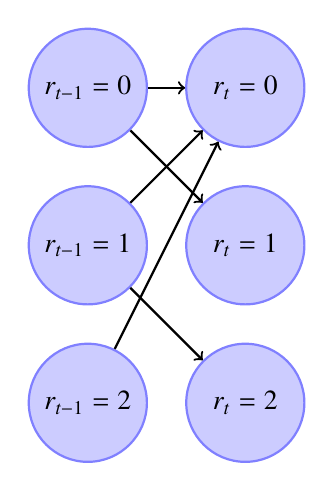
\begin{tikzpicture}
\tikzstyle{every node} = [circle,draw=blue!50,fill=blue!20,thick,
inner sep=0pt,minimum size=15mm]
\node (a) at (-1, 2) {$r_{t-1}=0$};
\node (b) at (-1, 0) {$r_{t-1}=1$};
\node (c) at (-1, -2) {$r_{t-1}=2$};
\node (d) at (1, 2) {$r_t=0$};
\node (e) at (1, 0) {$r_t=1$};
\node (f) at (1, -2) {$r_t=2$};
\draw [->,thick] (a) -- (d);
\draw [->,thick] (a) -- (e);
\draw [->,thick] (b) -- (d);
\draw [->,thick] (b) -- (f);
\draw [->,thick] (c) -- (d);
\end{tikzpicture}
\caption{Example of possible transitions for $r_{t-1}$.}
\label{fig:transition}
\end{figure}

For the computation of the predictive distribution, we first note that it is
only dependent on the data of the current segment $\mathbf{z}^{r_{t-1}}=
[\mathbf{z}_{t-1}]$ in case $r_{t-1}=0$ and $\mathbf{z}^{r_{t-1}}=
[\mathbf{z}_{t-1-r_{t-1}},\dots,\mathbf{z}_{t-1}]$ otherwise. Thus, it can
be expressed as $p(\mathbf{z}_t\mid r_{t-1}, \mathbf{z}^{r_{t-1}})$. We finally
introduce the model parameters $\boldsymbol{\eta}^{r_{t-1}}$ that are learned
on the current segment. We compute the predictive distribution by marginalizing
out the model parameters $\boldsymbol{\eta}^{r_{t-1}}$, i.e.

\begin{eqnarray}
\label{eqn:preddistr}
p(\mathbf{z}_t\mid r_{t-1},\mathbf{z}^{r_{t-1}},\boldsymbol{\psi}^{r_{t-1}})
&=&\nonumber\\\int_{\boldsymbol{\eta}^{r_{t-1}}}
p(\mathbf{z}_t\mid\boldsymbol{\eta}^{r_{t-1}})p(\boldsymbol{\eta}^{r_{t-1}}\mid
r_{t-1},\mathbf{z}^{r_{t-1}},\boldsymbol{\psi}^{r_{t-1}})
d\boldsymbol{\eta}^{r_{t-1}}.
\end{eqnarray}

Here, we added the prior hyperparameters $\boldsymbol{\psi}^{r_{t-1}}$ for
completeness. The integral in \eqref{eqn:preddistr} can be solved analytically
if we model the prior of the parameter vector $\boldsymbol{\eta}^{r_{t-1}}$ as a
conjugate to the probability density function $p(\mathbf{z}_t\mid
\boldsymbol{\eta}^{r_{t-1}})$. Otherwise, this leads to expensive numerical
computations. When the terms inside the integral are conjugate models, the
marginal distribution is usually a function of the sufficient statistics which
can be updated iteratively as data arrives.

\subsection{Complexity and Approximate Inference}
In order to exactly infer the positions of all change-points until time $t$, we
need to compute and store $p(r_t\mid \mathbf{z}_{1:t})$ for $t$ and all previous
time steps. We can then get the Maximum A Posteriori (MAP) estimate of the
sequence of segment lengths using the on-line Viterbi
algorithm of~\cite{fearnhead07online}.

Regarding complexity, if we have processed $n$ data points, the storage of the
full posterior distribution has a memory cost of $O(n^2)$ and $O(n)$
computational cost. This might be prohibitive for huge datasets. For this
reason, the distribution has to be approximated. A simple way sketched
in~\cite{adams07bayesian} is to discard values where the distribution is
significantly low, i.e., lower than a given threshold. However, as we want to
accurately estimate our distribution and control the computational costs, we use
a \emph{particle filter}. The state-space of $r_t$ being discrete and the number
of successor states being small, we can evaluate all the possible descendants of
$r_t$. Indeed, if $r_t$ has $k$ possible values, $r_{t+1}$ will have $k+1$
possible values. At each time step $t$, we approximate the posterior
distribution with a set $\{r_t^{(i)},\boldsymbol{\psi}^{r_{t-1},(i)}\}_{i=1}^M$ of
$M$ particles weighted by $\{w_t^{(i)}\}_{i=1}^M$ with

\begin{equation}
\label{eqn:weight}
w_t^{(i)} \propto p(\mathbf{z}_t\mid r_{t-1}^{(i)},\mathbf{z}^{r_{t-1},(i)},
\boldsymbol{\psi}^{r_{t-1},(i)}).
\end{equation}

In order to limit the number of particles at each time step, we use the
Stratified Optimal Re-sampling (SOR) presented in~\cite{fearnhead07online},
whenever $M$ gets bigger than our particles number limit $P$.

Using this method reduces the memory costs to $O(n)$ and the computational costs
to $O(1)$, i.e. constant run-time. We also notice that this particle filter is
Rao-Blackwellized~\cite{casella96rao} and has thus a lower variance since the
sampling space of the state is reduced to $r_t$ and the rest is marginalized out.

\subsection{Application to Motion Data Segmentation}
In our particular case, data comes from an IMU and we consider accelerations in
the three standard axes $x,y,z$, with $x$ pointing forward, $y$ on the left, and
$z$ upward. We can safely assume that an IMU measurement $\mathbf{z}_t$ arises
from a multivariate normal distribution with mean $\boldsymbol{\mu}_n$ and
covariance matrix $\boldsymbol{\Sigma}_n$ for segment $s_n$. The parameter
vector for segment $r_t$ is thus $\boldsymbol{\eta}^{r_{t}}=
\{\boldsymbol{\mu}^{r_{t}},\boldsymbol{\Sigma}^{r_{t}}\}$. In order to solve
the integral in (\ref{eqn:preddistr}) analytically, we model the parameter prior
as a normal-Wishart distribution which is conjugate to the multivariate
Gaussian. This distribution has four hyperparameters
$\boldsymbol{\psi}^{r_{t}}=\{\kappa^{r_{t}},\boldsymbol{\rho}^{r_{t}},
\nu^{r_{t}},\boldsymbol{\Lambda}^{r_{t}}\}$ that can be updated iteratively
as a new data point $\mathbf{z}_t$ arrives with:

\begin{eqnarray}
\label{eqn:hyperupdate}
\kappa^{r_{t}}&=&\kappa^{r_{t-1}}+1\nonumber\\
\boldsymbol{\rho}^{r_{t}}&=&\frac{\kappa^{r_{t-1}}\;
\boldsymbol{\rho}^{r_{t-1}}+\mathbf{z}_t}{\kappa^{r_{t-1}}+1}\nonumber\\
\nu^{r_{t}}&=&\nu^{r_{t-1}}+1\nonumber\\
\boldsymbol{\Lambda}^{r_{t}}&=&\boldsymbol{\Lambda}^{r_{t-1}}+
\frac{\kappa^{r_{t-1}}}{\kappa^{r_{t-1}} + 1}
(\mathbf{z}_t - \boldsymbol{\rho}^{r_{t-1}})
(\mathbf{z}_t - \boldsymbol{\rho}^{r_{t-1}})^\intercal.
\end{eqnarray}

In case we start a new segment and $r_t=0$, the hyperparameters are fixed to
some prior values.

From (\ref{eqn:hyperupdate}), we can express the parameters of the
multivariate normal distribution as

\begin{eqnarray}
\label{eqn:ssmvn}
\boldsymbol{\mu}^{r_{t}}&=&\boldsymbol{\rho}^{r_{t}}\nonumber\\
\boldsymbol{\Sigma}^{r_{t}}&=&\text{inv}(\boldsymbol{\Lambda}^{r_{t}})/\kappa^{r_{t}}.
\end{eqnarray}

Finally, for the computation of the predictive distribution in
\eqref{eqn:preddistr}, we approximate the multivariate normal distribution with
a Student's $t$-distribution which is known to be more robust to outliers in
case of few data points. This distribution converges to the Gaussian when its
degrees of freedom go to infinity. We use the number of processed points as the
degrees of freedom for the distribution, so as to have a bigger variance at the
beginning.


\section{Labeling of Traffic Situations\label{sec:labeling}}
Our aim is to find a label for each segmented motion pattern. This label
represents a traffic situation, e.g., a stop or turn condition. Moreover, we are
interested in associating two different motion segments to the same label
whenever they depict the same traffic situation. In the following, we show how
we can integrate this labeling into the on-line framework of
Section~\ref{sec:motion}.

\subsection{Traffic Situation Model}
As shown above, we denote the label of a segment $r_t$ as $l_t$. This label can
take values in $[1,2,\dots,N]$ corresponding to $N$ parametric models $M_1,M_2,
\dots,M_N$. Each of the $M_i$ is a generative model $p(\mathbf{c}_t\mid
\boldsymbol{\eta}_i)$ for a particular traffic situation with parameter vector
$\boldsymbol{\eta}_i$. At time $t$, we estimate the distribution over the known
models conditioned on the data seen so far and the segment we are in with Bayes
law as

\begin{eqnarray}
\label{eqn:labeling}
p(l_t\mid r_t,\mathbf{c}_{1:t})&\propto&p(\mathbf{c}_{1:t}\mid l_t,r_t)
p(l_t\mid r_t)\nonumber\\
&=& p(\mathbf{c}^{r_t}\mid l_t,r_t)p(l_t\mid r_t),
\end{eqnarray}

where $\mathbf{c}^{r_t}$ represents data on the current segment $r_t$.

For the prior part in \eqref{eqn:labeling}, we use the posterior of the previous
time step, that is
$p(l_t\mid r_t)=p(l_{t-1}\mid r_{t-1},\mathbf{c}^{r_{t-1}})$. If we are in a new
segment with $r_t=0$, we set the prior to a uniform distribution over the known
models, i.e., $p(l_t=1:N\mid r_t)=\frac{1}{N}$. The likelihood part in
\eqref{eqn:labeling} is computed with the model probability density function
$p(\mathbf{c}_t\mid \boldsymbol{\eta}_i)$ in the same fashion as in
\eqref{eqn:preddistr}, i.e., using a conjugate prior with hyperparameters
$\boldsymbol{\psi}_i$ as will be detailed below.

As we want to be able to discover new traffic situations on-line, we have to
state if the current data $\mathbf{c}_t$ is unlikely to come from any of the
$N$ known models so far. Following the strategy of~\cite{ranganathan10pliss},
we perform $N$ likelihood ratio test at each time step. We compare model $M_i$
with a model learned over segment $r_t$. The test statistic is

\begin{equation}
\label{eqn:statistic}
D = -2\ln\frac{p(\mathbf{c}_t\mid \boldsymbol{\psi}_i)}{p(\mathbf{c}_t\mid
\boldsymbol{\psi}^{r_t})},
\end{equation}

where $\boldsymbol{\psi}^{r_t}$ is the maximum likelihood solution for
$\boldsymbol{\psi}$ over the current segment $r_t$.

Based on the value of $D$, we have to decide whether to accept or reject the
null hypothesis, i.e., data in segment $r_t$ arises from model $M_i$. It is
shown that when the sample size grows towards infinity, $D$ converges towards a
Chi-square distribution with $K-1$ degrees of freedom, where $K$ is the
dimension of $\boldsymbol{\psi}$. In our case, the sample size represents the
number of data used to compute the maximum likelihood solution. As will be
shown below, it will be sufficient to approximate $D$ with a Chi-square
distribution. We will thus compare $D$ to the Chi-square value corresponding to
the desired statistical significance $\xi$ of the null hypothesis. In practice,
this is done by computing the value of the cumulative distribution
function of the Chi-square distribution for $D$ and reject the model
$M_i$ if it is below $\xi$.

In case all models are rejected, we create a new instance $M_{N+1}$
with hyperparameter vector $\boldsymbol{\psi}^{r_t}$, set $p(l_t=N+1\mid r_t,
\mathbf{c}^{r_t})=p_{new}$, and $p(l_t=1:N\mid r_t,\mathbf{c}^{r_t})=
(1-p_{new})/N$. We update the hyperparameters $\boldsymbol{\psi}_i$ of model
$M_i$, such that $i=\argmax_{j=1:N}p(l_t=j\mid
r_t,\mathbf{c}^{r_t})$, with $\mathbf{c}_t$.

From an implementation point of view, we attach the distribution
\eqref{eqn:labeling}, the hyperparameters $\boldsymbol{\psi}^{r_t}$, and the
incremental set of known models $M_i$ to each particle. Thus, our system is able
to learn new traffic situations on-line and refine its knowledge over
previously visited scenes.

\subsection{Measurements Representation}
We represent images using the widely adopted \emph{bag-of-words}
model~\cite{sivic03video}. In the document modeling formulation, text documents
are represented as histograms of word counts from a given dictionary. This model
can be easily applied to computer vision tasks, words being replaced by features
and text documents by images.

We use Scale-Invariant Feature Transform (SIFT)~\cite{lowe04distinctive}
descriptors computed at Difference of Gaussians (DoG) keypoints. SIFT
descriptors have been shown to be highly discriminative for object recognition.
Although some authors claim that they obtain better results with dense grid
representations~\cite{feifei05bayesian}, DoG interest points are more suitable
for our purpose. Indeed, we are not interested in capturing uniform regions such
as sky, but rather focused on objects. $N$ images are randomly selected from the
entire dataset to build a \emph{codebook} or dictionary of features using
K-means clustering. Each feature of an image is then assigned to the nearest
\emph{codeword} of the dictionary and we can therefore build a convenient
histogram representation.

The link between bag-of-\emph{features} models in computer vision and
bag-of-words models in text document modeling is intuitive. We can therefore use
the generative model of~\cite{madsen05modeling} to represent an image in a
probabilistic manner as was already proposed in~\cite{ranganathan09bayesian}.
The idea of~\cite{madsen05modeling} is to represent a text document with a
Dirichlet Compound Multinomial (DCM) model, also known as multivariate Polya
distribution. It models the fact that when a particular word occurs in a
document, it is more likely to appear again. In terms of images, this makes
sense since the same feature is likely to appear several times in the same
image. Furthermore, the DCM combines a multinomial model and a Dirichlet prior,
and provides an analytical solution to the marginalization of the multinomial
parameters. The multinomial distribution $p(\mathbf{c}_t\mid
\boldsymbol{\theta})$ has parameters $\boldsymbol{\theta}=[\theta_1,\theta_2,
\dots,\theta_K]$, corresponding to $\boldsymbol{\eta}$ above. The Dirichlet
prior $p(\boldsymbol{\theta}\mid\boldsymbol{\alpha})$ has hyperparameters
$\boldsymbol{\alpha}=[\alpha_1,\alpha_2,\dots,\alpha_K]$, corresponding to
$\boldsymbol{\psi}$ above. The likelihood part of \eqref{eqn:labeling} can now
be formulated as

\begin{eqnarray}
\label{eqn:polya}
p(\mathbf{c}^{r_t}\mid l_t,r_t,\boldsymbol{\alpha}^{r_t})&=&
\int_{\boldsymbol{\theta}}
p(\mathbf{c}^{r_t}\mid\boldsymbol{\theta})p(\boldsymbol{\theta}\mid
l_t,r_t,\boldsymbol{\alpha}^{r_t})d\boldsymbol{\theta}\\\nonumber
&=&\frac{n!}{\prod_{k=1}^K n_k!}\frac{\Gamma(\alpha^{r_t})}
{\Gamma(n+\alpha^{r_t})}\prod_{k=1}^K\frac{\Gamma(n_k+\alpha^{r_t}_k)}
{\Gamma(\alpha^{r_t}_k)},
\end{eqnarray}

where $\Gamma(.)$ is the Gamma function, $n_k=\sum_{j=t-r_t}^t
\mathbf{c}_j\,(k)$, $n=\sum_{k=1}^K n_k$,
$\alpha^{r_t}=\sum_{k=1}^K\alpha^{r_t}_k$, and we added the hyperparameter
$\boldsymbol{\alpha}^{r_t}$ in the conditional.

As there exists no analytical solution to the maximum likelihood parameters
estimation of a DCM, an iterative gradient descent
optimization~\cite{minka03estimating} is used and leads to the update rule

\begin{equation}
\label{eqn:alpha_update}
\alpha_k^{r_t} = \alpha^{r_{t-1}}_k\frac{\sum_{j=t-r_t}^t\Psi(n_{jk}+
\alpha^{r_{t-1}}_k)-\Psi(\alpha^{r_{t-1}}_k)}{\sum_{j=t-r_t}^t\Psi(n_j+
\alpha^{r_{t-1}})-\Psi(\alpha^{r_{t-1}})},
\end{equation}

where $\Psi(.)$ is the digamma function, $n_{jk}=\mathbf{c}_j\,(k)$, and
$n_j=\sum_{k=1}^K n_{jk}$.


\section{Action Model\label{sec:action}}
We want to estimate the posterior probability distribution over actions
conditioned on the current traffic situation and segment. To this end, we
closely follow the strategy of Section~\ref{sec:labeling}. To each of the
traffic situation model $M_i$ is associated an action model $A_i$, which we fit
with a Gaussian Mixture Model (GMM). For the same traffic situation $M_i$, we
are able to model several possible behaviors corresponding to the different
Gaussian components. For instance, when we reach a traffic light, we might brake
when the light is red and continue when it is green. Moreover, a driver does not
always brake or accelerate exactly the same manner every time. Finally, our
system can adapt to new drivers. We can thus formulate the following model that
we estimate and update at each time step:

\begin{equation}
\label{eqn:action}
p(\mathbf{a_t} \mid r_t, l_t,\mathbf{z}_{1:t},\boldsymbol{\psi}^{\mathbf{x}_t})=
\sum_{\mathbf{x}_t} p(\mathbf{x}_t)p(\mathbf{a}_t\mid\mathbf{x}_t,r_t,l_t,
\mathbf{z}_{1:t},\boldsymbol{\psi}^{\mathbf{x}_t}),
\end{equation}

where $\mathbf{x}_t$ is a $K$-dimensional vector with a single one at the
position $k$ encoding for the $k$-th Gaussian and zeros elsewhere,
$p(\mathbf{x}_t)$ is the prior for selecting a particular Gaussian component
$\mathbf{x}_t$, and $p(\mathbf{a}_t\mid\mathbf{x}_t,r_t,l_t,
\mathbf{z}_{1:t},\boldsymbol{\psi}^{\mathbf{x}_t})$ is a Gaussian distribution
with hyperparameters $\boldsymbol{\psi}^{\mathbf{x}_t}$. In a similar fashion as
in Section~\ref{sec:motion}, we have marginalized out the parameters of the
Gaussian and we are thus able to iteratively update the hyperparameters. The
prior distribution $p(\mathbf{x}_t)$ is defined as

\begin{equation}
\label{eqn:gaussianprior}
p(\mathbf{x}_t(i)=1)\propto n_t^i,
\end{equation}

where $n_t^i$ is the sum of the points assigned to Gaussian component $i$.

Upon reception of a new data point $\mathbf{z}_t$, we perform the likelihood
ratio test on all the Gaussian components $\mathbf{x}_{t-1}$ of the model $l_t$.
Compared to the method proposed in Section~\ref{sec:labeling}, the Chi-square
assumption does not hold and we directly threshold the ratio with $\varepsilon$.
If all the components are rejected, a new Gaussian is created with
hyperparameters $\boldsymbol{\psi}_0$. We update the hyperparameters of the most
likely Gaussian component with the rule from \eqref{eqn:hyperupdate} and
increment the corresponding $n_t^i$.

From an implementation point of view, the distribution~\eqref{eqn:action} and
the learned GMM $A_i$ are attached to the particle filter of
Section~\ref{sec:motion}.


\section{Experiments\label{sec:exp}}
In order to evaluate the approach proposed in this paper, we have collected
a dataset with a car in an urban setting. Our car is equipped with a Sony
XCD-SX910 camera recording $1280$x$960$ images at $3.75$ frames per second and
an XSens MTi IMU running at $100$ Hz with $x$ pointing forward, $y$ to the
right, and $z$ upward. The sequence contains $8218$ images and lasts around $40$
minutes. We have encountered different scenes comprising of traffic lights,
crosswalks, or changes of speed limit. We have driven in a loop so as to come
several times in the same situation and thus have an estimation of the quality
of our solution.

In the rest of this Section, we first display an experiment of the whole
algorithm on synthetic data. It is easier to have a ground truth on simulated
data and hence validate our approach. We then show results on real-world data
with a detailed analysis of all the components.

\subsection{Simulation}
For visualization purposes, we have simulated IMU data with an univariate normal
distribution and have introduced change-points every $50$ data points. We have
randomly generated 3 different $\boldsymbol{\alpha}_i$ with $K=256$ coding for
the traffic situations. Although the algorithm starts with no prior knowledge,
we could also start with previously learned models $M_i$ and $A_i$.

Fig.~\ref{fig:simulation} depicts the output of the simulation and demonstrates
the pertinence of our method. After a change-point, the algorithm needs a time
of adaptation to collect enough data points in order to converge to the correct
prediction. In Fig.~\ref{fig:simulation}, we display the MAP solution for
\eqref{eqn:action} on the bottom plot and thus the prediction reflects the
Gaussian component with the biggest number of data points. The code runs in
MATLAB with no attempt for optimization and has a processing time of about
$0.3$ seconds per time step. In a realistic scenario, histogram building from
image adds up to the time.

\begin{figure}[t]
\centering
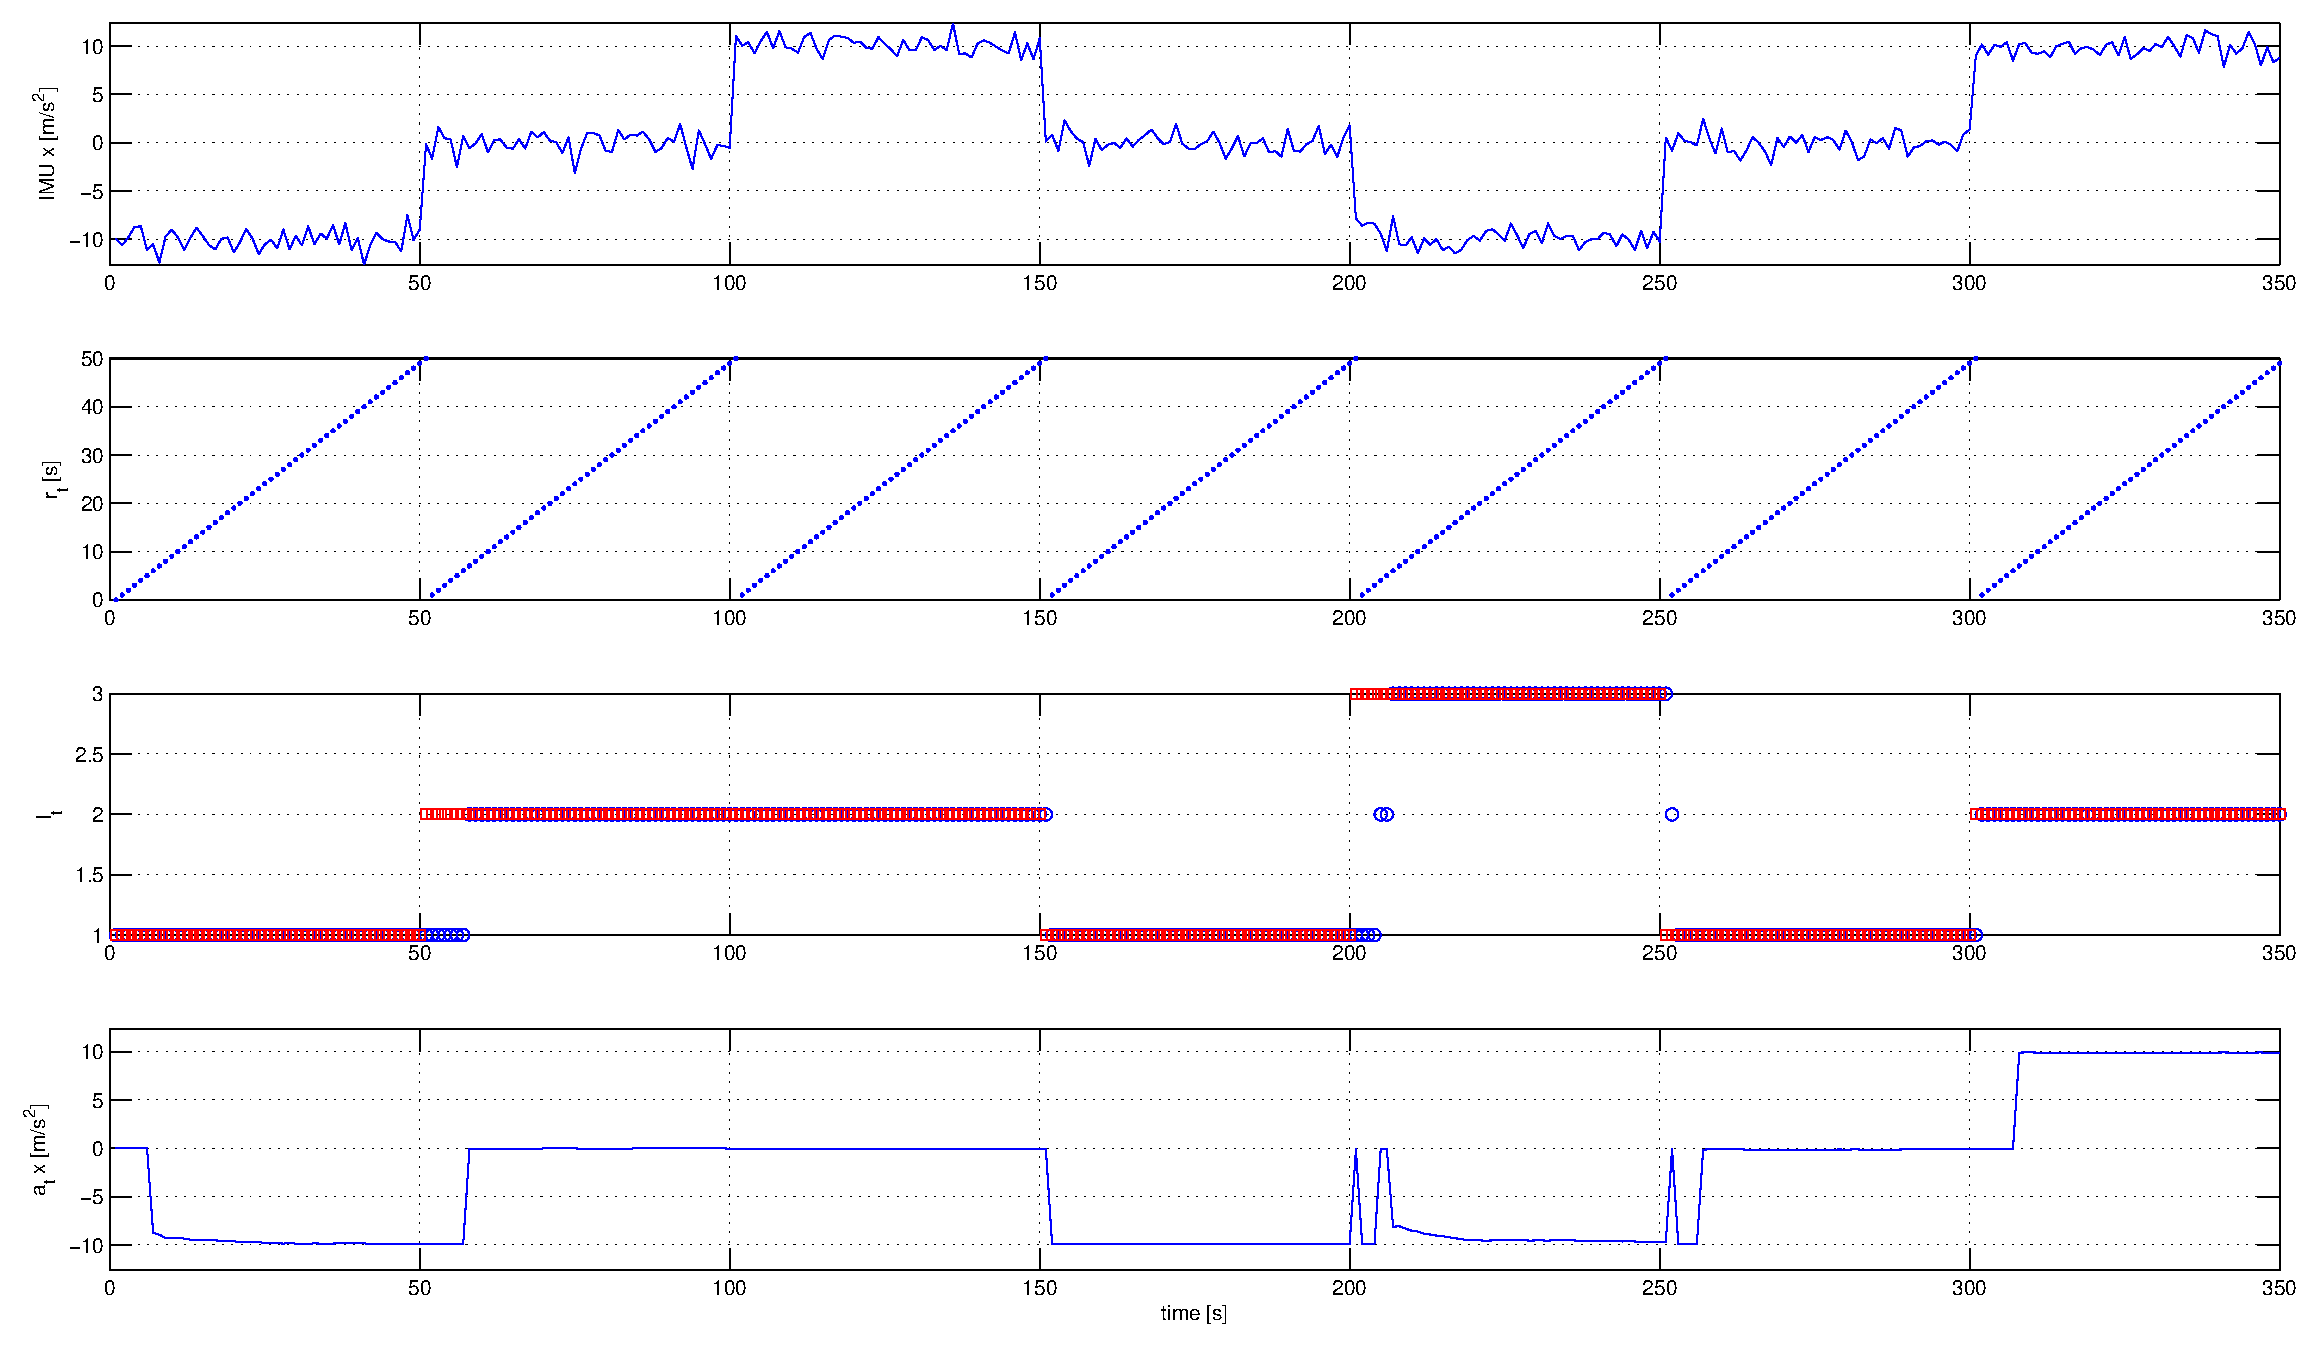
\includegraphics[width=\columnwidth]{fig/simResult.eps}
\caption{Simulation results of the entire algorithm. From top to bottom, the
plots display the simulated IMU data $\mathbf{z}_t$, the inferred segment
lengths $r_t$, the inferred labels $l_t$ (blue circle) and ground truth
(red square), and the MAP for $\mathbf{a}_t$.}
\label{fig:simulation}
\end{figure}

\subsection{Motion Segmentation}
In this experiment, we want to estimate the quality of our motion segmentation
algorithm from Section~\ref{sec:motion}. We performed inference on the
final posterior distribution \eqref{eqn:joint} to get the optimal
sequence of segment lengths which represents our motion segments. We set the
hazard rate to $\lambda=1/10$, the number of particles to $P=100$, and the prior
hyperparameters of the normal-Wishart to $\kappa_0=1,
\boldsymbol{\rho}_0=\mathbf{0},\nu_0=3,\boldsymbol{\Lambda}_0=\mathbf{I}$. We
only considered IMU data at $10$ Hz.

Fig.~\ref{fig:motion_segments} shows the extracted motion segments along with
the corresponding IMU data. Our algorithm identified $165$ segments which are
validated by visual inspection of the IMU data. Furthermore, the segmentation
has been compared to a manual annotation of our image sequence and exhibited an
accuracy of approximatively $92\%$. For the labeling of the change-points, we
have watched the video and noted down where we would expect a change of driving
behavior. The parameter $\lambda$ controls the false positives/negatives rates.
As expected, the typical motion patterns that appeared were driving straight
with no acceleration, driving straight with acceleration or deceleration, and
turning left or right.

\begin{figure}[t]
\centering
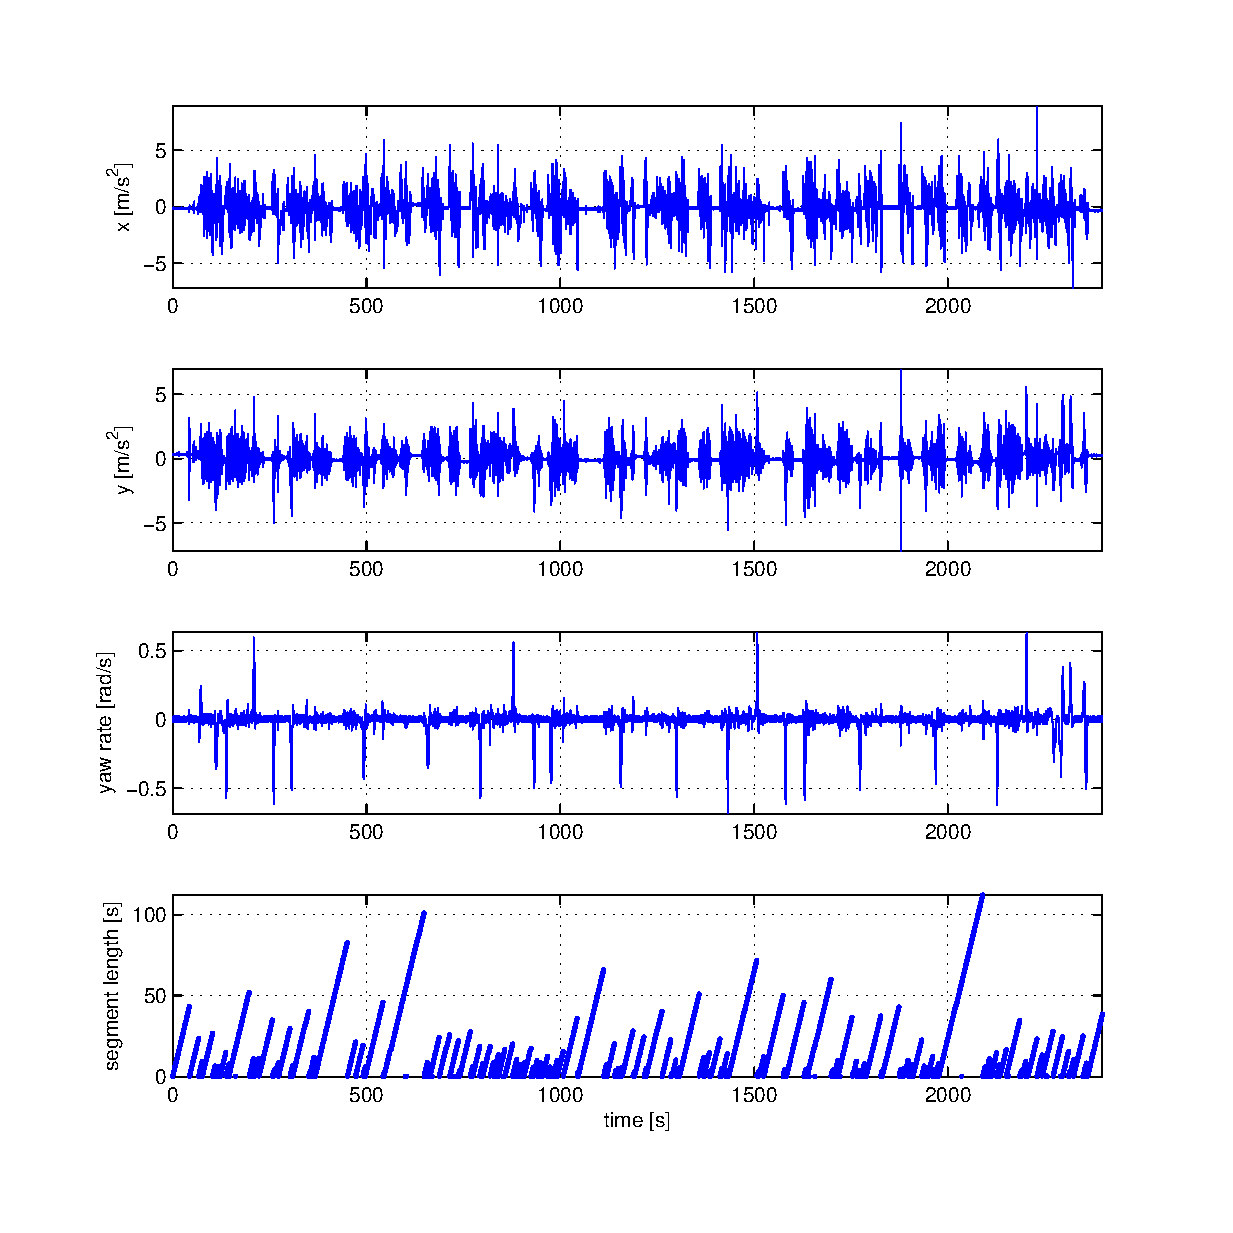
\includegraphics[width=\columnwidth]{fig/cpResult.eps}
\caption{Optimal motion segmentation from IMU data. The three top plots are the
IMU raw values over time. The bottom plot depicts the motion segments
discovered by our algorithm.}
\label{fig:motion_segments}
\end{figure}

\subsection{Traffic Situation Labeling and Recognition}
In this experiment, we are interested in evaluating the part of our algorithm
presented in Section~\ref{sec:labeling} and perform inference on
\eqref{eqn:labeling}. In a first phase, we collected a subset
of images from traffic lights, yield signs, pedestrian crossings, and regular
straight roads. Models $M_i$ were learned on these images and frozen during the
evaluation. In a second phase, we started the algorithm with no prior models.
The dictionary was created from a set of $N=400$ randomly picked images and the
SIFT features quantized into $K=256$ visual words.

ANOTHER PARAGRAPH SHOWING AND EXPLAINING THE RESULTS. IF SPACE, SHOW A GRAPH.

\subsection{Action Prediction}
FIRST PARAGRAPH DESCRIBING THE EXPERIMENTAL CONDITIONS.

SECOND PARAGRAPH OUTPUTTING AND COMMENTING THE RESULTS.


\section{Conclusion\label{sec:conc}}
In this paper, we have presented a novel approach to on-line learning of driving
behaviors. To this end, we have developed an entire Bayesian framework that is
able to learn and adapt to new situations. For computational and storage
purposes, we have approximated the full posterior distribution with a
Rao-Blackwellized particle filter. We have shown an original application of the
change-point detection model of~\cite{adams07bayesian} and
\cite{fearnhead07online} to the segmentation of IMU data with a clearer
formulation. Visual traffic situations models have been learned
probabilistically from images and linked to an action model from IMU data. Our
system is suitable for lifelong learning since it is able to continuously update
its models. We have conducted experiments on a challenging urban dataset and
validated our approach.

In the near future, we aim at improving our image representation with a more
sophisticated model. In particular, we want to consider images as an histogram
of objects rather than features. We aspire to determine which objects in the
scene influence an action. Our second mid-term goal is to deploy our system in
a car and have a real-time driving assistant.


\section*{Acknowledgment}
This work has partly been supported by the EC under FP7-231888-EUROPA and by the
DFG under SFB/TR-8.

\bibliographystyle{sty/IEEEtran}
\bibliography{bib/IEEEabrv,bib/bibliography}

\end{document}
